\chapter{Appendix}

\section{Poisson noise  \label{app:poisson}}
%=========================
Assume that the expected amount of measured photons per unit time equals $r$.
Let us now divide this unit of time in a $k$ time intervals. If $k$ is
sufficiently large, the time intervals are small, so the probability of
detecting a photon in such an interval is small, and the probability of
detecting two or more is negligible. Consequently, we can assume that in every
possible measurement, only zero or one photon is detected in every
interval. The probability of detecting one photon in an interval is then $r /
k$. A measurement of $n$ photons must consist of $n$ intervals with one
photon, and $k - n$ intervals with no photons. The probability of such a
measurement is:
\begin{equation}
p_r(n) = \left( \frac{r}{k} \right)^n \left(1 - \frac{r}{k} \right)^{k-n}
       \frac{k!}{n!(k-n)!}  \label{jn:poisson:1}
\end{equation}
The first factor is the probability of detecting $n$ photons in $n$ intervals.
The second factor is the probability of detecting no photons in $n - k$
intervals.  The third factor is the amount of ways that these $n$ successful
and $n-k$ unsuccessful intervals can be combined in different measurements.

As mentioned above, equation (\ref{jn:poisson:1}) becomes better when $k$ is
larger.  To make it exact, we simply have to let $k$ go to infinity.
\begin{equation}
  \lim_{k \rightarrow \infty} p_r(n) 
  = \frac{r^n}{n!} \lim_{k \rightarrow \infty} \left( 1 - \frac{r}{k} \right)^k
\end{equation}
It turns out that computing the limit of the logarithm is easier, so we have
\begin{eqnarray}
  \lim_{k \rightarrow \infty} \left( 1 - \frac{r}{k} \right)^k
 & = &
 \exp \left(\lim_{k \rightarrow \infty} \frac{\ln(k - r) - ln(k)}{1/k}  \right)
\nonumber\\
& = & 
  \exp \left(\lim_{k \rightarrow \infty}  
  \frac{1/ (k-r) - 1/k}{-1/k^2} \right) \nonumber \\
& = & \exp (-r)
\end{eqnarray}
So it follows that 
\begin{equation}
  \lim_{k \rightarrow \infty} p_r(n) = \frac{e^{-r} r^n}{n!}. 
\end{equation}

\newpage
\section{Convolution and PSF\label{app:convolution}}
%=========================
In section \pref{sec:collimation}, the collimator point spread function (PSF)
was computed. The collimator PSF tells us which image is obtained for a point
source at distance $H$ from the collimator. What happens if two point sources
are positioned in front of the camera, both at the same distance $H$? Since
the sources and the photons don't interact with each other, all what was said
above still applies, for each of the sources. The resulting image will consist
of two PSFs, each centered at the detector point closest to the point
source. Where the PSFs overlap, they must be added, since the detector area
in the overlap region gets photons from both sources. The same is true for
three, four, or one million point sources, all located at the same distance
$H$ from the collimator. To predict the image for a set of one million point
sources, simply calculate the corresponding PSFs centered at the
corresponding positions on the detector, and sum everything.

The usual mathematical description of this can be considered as a two step
approach:
\begin{enumerate}
\item
Assume that the system is perfect: the image of a point source is a point,
located on the perpendicular projection line through the point source.
Mathematicians would call that ``point'' in the image a ``Dirac impulse''.
The image of two or more point sources contains simply two or more Dirac
impulses, located at corresponding projection lines.\\
%
Let $f(x,y)$ represent the image value at position $(x,y)$. This image
can be regarded as the sum of an infinite number of Dirac impulses
$\delta(x,y)$, one at every location $(x,y)$:
\begin{eqnarray}
f(x,y) & = & (f \otimes \delta) (x,y)\\
       & = & \intii du \intii dv \, f(u,v) \, \delta(x-u, y-v)
\end{eqnarray}

\item
Correction of the first step: the expected image of a point is not a Dirac
impulse, but a PSF. Therefore, replace each of the Dirac impulses in the image
by the corresponding PSF, centered at the position of the Dirac impulse.
\begin{eqnarray}
g(x,y) & = & (f \otimes \mbox{PSF}) (x,y)\\
       & = & \intii du \intii dv \, f(u,v) \, \mbox{PSF}(x-u, y-v)
\end{eqnarray}
\end{enumerate}

The second operation is called the {\em convolution} operation. Assume that a
complex flat (e.g. a inhomogeneous radioactive sheet) tracer distribution
would be put in front of the camera, parallel to the collimator (at distance
$H$). What image will be obtained?  Regard the distribution as consisting of
an infinite number of point sources. This does not change the distribution, it
only changes the way you look at it. Project all of these sources along an
ideal perpendicular projection line into the image. You will now obtain an
image consisting of an infinite number of Dirac impulses. Replace each of
these impulses with the PSF and sum the overlapping values to obtain the
expected image.

If the distance to the collimator is not the same for every point source, then
things get more complicated. Indeed, the convolution operator assumes that the
PSF is the same for all point sources. Therefore, to calculate the expected
image, the previous procedure has to be applied individually for every
distance, using the corresponding distance dependent PSF. Finally, all
convolved images have to be summed to yield the expected image.

\newpage
\section{Combining resolution effects: convolution of
two Gaussians \label{app:convol2gauss}}
%=========================
Very often, the PSF can be well approximated as a Gaussian. This fact comes in
handy if we want to combine two PSFs. For example: what is the combined effect
of the intrinsic resolution (PSF of scintillation detection) and the collimator
resolution (collimator PSF)?

How can two PSFs be combined? The solution is given in appendix
\pref{app:convolution}: one of the PSFs is regarded as a collection of Dirac
impulses. The second PSF must be applied to each of these pulses. So we must
compute the convolution of both PSFs. This appendix shows that if both are
approximately Gaussian, the convolution is easy to compute.

Let us represent the first and second PSFs as follows:
\begin{equation}
  F_1(x) = A \exp\left( -\frac{x^2}{a^2}\right)  \;\;\; \mbox{and} \;\;\;
  F_2(x) = B \exp\left( -\frac{x^2}{b^2}\right)
\end{equation}
Thus, $\sigma_1 = a / \sqrt{2}$ and $A = 1 / (\sqrt{2 \pi} \sigma_1)$, and
similar for the other PSF. The convolution is then written as:
%
\begin{eqnarray}
(F_1 \otimes F_2)(x) & = &
  AB \intii \exp\left(- \frac{u^2}{a^2} - \frac{(x-u)^2}{b^2}\right) du\\
& = & AB \intii \exp\left(- m u^2   + \frac{2xu}{b^2} - \frac{x^2}{b^2}\right)
  du \\
m & = & \left( \frac{1}{a^2} + \frac{1}{b^2}\right)
\end{eqnarray}
%
The exponentiation contains a term in $u^2$ and a term in $u$. We can get rid of
the $u$ by requiring that both terms result from squaring something of the
form $(u + C)^2$, and rewriting everything as $(u + C)^2 - C^2$. The $C^2$ is
not a function of $u$, so it can be put in front of the integral sign.
% 
\begin{eqnarray}
 (F_1 \otimes F_2)(x)  &  = & AB \intii \exp\left(- \left( \sqrt{m} u 
         - \frac{x}{b^2 \sqrt{m}} \right)^2
       + \frac{x^2}{b^4 m}
       - \frac{x^2}{b^2}\right) du\\
 & = &  AB \exp\left(\frac{x^2}{b^4 m} - \frac{x^2}{b^2}\right)
     \intii \exp\left(- \left( \sqrt{m} u 
         - \frac{x}{b^2 \sqrt{m}} \right)^2\right) du
\end{eqnarray}
The integrand is a Gaussian. The center is a function of $x$, but the standard
deviation is not. The integral from $-\infty$ to $\infty$ of a Gaussian is a
finite value, only dependent on its standard deviation. Consequently, the
integral is not a function of $x$. Working out the factor in front of the
integral sign and combining all constants in a new constant $D$, we obtain
%
\begin{equation}
 (F_1 \otimes F_2)(x) =  D \exp\left(-\frac{x^2}{a^2 + b^2}\right)
\end{equation}
%
So the convolution of two Gaussians is again a Gaussian. The variance of the
resulting Gaussian is simply the sum of the input variances (by definition, the
variance is the square of the standard deviation).

The FWHM of a Gaussian is proportional to the standard deviation, so we obtain
a very simple expression to compute the FWHM resulting from the convolution of
multiple PSFs:
\begin{equation}
 \mbox{FWHM}^2 = \mbox{FWHM}_1^2 + \mbox{FWHM}_2^2 + \ldots + \mbox{FWHM}_n^2
\end{equation}

\newpage
\section{Error propagation \label{app:error}}
%==========================
The mean and the variance of a distribution $a$ are defined as:
\begin{eqnarray}
  \mbox{mean}(a) & = & \ol{a} = E(a) = \frac{1}{N} \sum_{i=1}^N a_i\\
  \mbox{variance}(a) & = & \sigma_a^2 = E\left[ (a - \ol{a})^2 \right]
   = \frac{1}{N} \sum_{i=1}^N (a_i - \ol{a})^2,
\end{eqnarray}
where $E$ is the expectation, $a_i$ is a sample from the distribution and the
summation is over the entire distribution. By definition, $\sigma_a$ is the
standard deviation. When computations are performed on samples from a
distribution (e.g. Poisson variables) the noise propagates into the
result. Consequently, one can regard the result also as a sample from some
distribution which can be characterized by its (usually unknown) mean value
and its variance or standard deviation. We want to estimate the variance of
that distribution to have an idea of the precision on the computed result. We
will compute the variance of the sum or difference and of the product of two
independent variables. We will also show how the variance on any function of
independent samples can be easily estimated using a first order approximation.

Keep in mind that these derivations only hold for {\em independent}
samples. If some of them are dependent, you should first eliminate them using
the equations for the dependencies.

\subsection{Sum or difference of two independent variables}
%----------------------------------------------
We have two variables $a$ and $b$ with mean $\ol{a}$ and $\ol{b}$
and variance $\sigma_a^2$ and $\sigma_b^2$. We compute $a \pm b$ and estimate
the corresponding variance $\sigma_{a \pm b}^2$.
\begin{eqnarray}
\sigma_{a \pm b}^2 & = & \E{\left((a \pm b) - (\ol{a} \pm \ol{b}) \right)^2}
           \nonumber\\
 & = & \E{(a-\ol{a})^2} + \E{(b-\ol{b})^2} \pm \E{2(a-\ol{a})(b-\ol{b})}
           \nonumber\\
 & = & \E{(a-\ol{a})^2} + \E{(b-\ol{b})^2} \pm 2 \E{(a-\ol{a})}\E{(b-\ol{b})}
           \nonumber\\
 & = & \sigma_a^2 + \sigma_b^2, \label{eq:app_sumerror}
\end{eqnarray}
because the expectation of $(a - \ol{a})$ is zero. The expectation
$\E{(a-\ol{a})(b-\ol{b})}$ is the covariance of $a$ and $b$. The
expectation of the product is the product of the expectations if the
variables are independent samples, and therefore, the covariance of
independent variables is zero.

So in linear combinations the noise adds up, even
if the variables are subtracted!

\subsection{Product of two independent variables}
%------------------------------------
For independent variables, the expectation of the product is the
product of the expectations, so we have:
\begin{eqnarray}
 \sigma_{ab}^2 & = & \E{\left( ab - \ol{a} \ol{b}\right)^2} \nonumber\\
  & = & \E{a^2b^2} + \ol{a}^2\ol{b}^2 - \E{2 a b \ol{a} \ol{b}} \nonumber\\
  & = & \E{a^2} \E{b^2} - \ol{a}^2 \ol{b}^2 \label{eq:app_noise_prod1}
\end{eqnarray}
This expression is not very useful, it must be rewritten as a function of
$\ol{a}$, $\ol{b}$, $\sigma_a$ and $\sigma_b$. To obtain that, we rewrite $a$
as $\ol{a} + (a - \ol{a})$:
\begin{eqnarray}
  \E{a^2} & = & \E{(\ol{a} + (a - \ol{a}))^2} \nonumber\\
 & = & \ol{a}^2 + \E{\left( a - \ol{a} \right)^2} + \E{2 \ol{a}(a - \ol{a})}
       \nonumber\\
 & = & \ol{a}^2 + \sigma_a^2
\end{eqnarray}
Substituting this result for $E[a^2]$ and $E[b^2]$ in
(\ref{eq:app_noise_prod1}) we obtain:
\begin{eqnarray}
\sigma_{ab}^2 & = & (\ol{a}^2 + \sigma_a^2)(\ol{b}^2 + \sigma_b^2) 
                     - \ol{a}^2 \ol{b}^2 \nonumber\\
 & = & \ol{a}^2\sigma_b^2 + \ol{b}^2\sigma_a^2 + \sigma_a^2 \sigma_b^2
        \nonumber\\
 & = & \ol{a}^2\ol{b^2}\left( \frac{\sigma_a^2}{\ol{a}^2} + 
       \frac{\sigma_b^2}{\ol{b}^2} 
     + \frac{\sigma_a^2\sigma_b^2}{\ol{a}^2\ol{b}^2}\right)\\
 & \simeq & \ol{a}^2\ol{b^2}\left( \frac{\sigma_a^2}{\ol{a}^2} + 
       \frac{\sigma_b^2}{\ol{b}^2}\right)
\end{eqnarray}
The last line is a first order approximation which is acceptable if the
relative errors are small. We conclude that when two variables are multiplied
the relative variances must be added. 

\subsection{Any function of independent variables}
%-----------------------------------------
If we can live with first order approximations, the variance of any function
of one or more variables can be easily estimated. Consider a function
$f(x_1, x_2, \ldots x_n)$ where the $x_i$ are independent samples from
distributions characterized by $\ol{x_i}$ and $\sigma_i$. Applying first order
equations means that $f$ is treated as a linear function:
\begin{eqnarray}
  \E{\left( f(x_1, \ldots x_n) - \E{f(x_1, \ldots x_n)}\right)^2}
  \simeq  \E{\left( f(x_1,\ldots x_n) 
        - f(\ol{x_1}, \ldots \ol{x_n})\right)^2} \nonumber \\
  \simeq  \E{\left( \left. \frac{\partial f}{\partial x_1} \right|_{\ol{x_1}}
                 (x_1 - \ol{x_1}) + \ldots
            \left. \frac{\partial f}{\partial x_n} \right|_{\ol{x_n}}
                 (x_n - \ol{x_n}) \right)^2} \nonumber \\
  = \left( \left. \frac{\partial f}{\partial x_1} \right|_{\ol{x_1}} \right)^2
        \sigma_1^2 + \ldots
    \left( \left. \frac{\partial f}{\partial x_n} \right|_{\ol{x_n}} \right)^2
         \sigma_n^2
\end{eqnarray}
The first step is a first order approximation: the expectation of a linear
function is the function of the expectations. Similarly, the second line is a
Taylor expansion, assuming all higher derivatives are zero. The third step is
the application of (\ref{eq:app_sumerror}).

With this approach you can easily verify that the variance on a product or
division is obtained by summing the relative variances.

\newpage
\section{Central slice theorem \label{app:cs}}
%=================================
This appendix gives a proof of eq (\pref{fouriertheorem}) for any angle
$\theta$. The projection $q(s,\theta)$ can be written as
\begin{equation}
  q(s, \theta) = \intii \lambda(s \cos\theta - r\sin\theta, 
                                s \sin\theta + r\cos\theta) dr
\end{equation}
The 1D Fourier transform of $q(s,\theta)$ along $s$ equals:
\begin{eqnarray}
  Q_1(\nu_s, \theta) &=& \intii q(s, \theta) e^{-j2\pi \nu_s s} ds 
    \nonumber\\
  &=& \intii\intii\lambda(s\cos\theta - r\sin\theta, 
                          s\sin\theta + r\cos\theta)e^{-j2\pi \nu_s s} dr ds
      \label{eq:Q1}
\end{eqnarray}
Now consider the 2D Fourier transform of $\lambda(x,y)$:
\begin{equation}
  \Lambda(\nu_x, \nu_y) = \intii \intii \lambda(x,y) 
       e^{-j2\pi (\nu_x x + \nu_y y)} dx dy
\end{equation}
We now switch to a rotated coordinate system by setting:
\begin{eqnarray}
   x = s \cos\theta - r\sin\theta \;\;\;&\mbox{and}& \;\;\;
   y = s\sin\theta + r\cos\theta\\
   \nu_x = \nu_s \cos\theta - \nu_r\sin\theta \;\;\;&\mbox{and}& \;\;\;
   \nu_y = \nu_s\sin\theta + \nu_r\cos\theta
\end{eqnarray}
It follows that $\nu_x x + \nu_y y = \nu_s s + \nu_r r$. The Jacobian
of the transformation equals unity, so $dx dy = dr ds$. Thus, we obtain:
\begin{eqnarray}
\lefteqn{\Lambda(\nu_s \cos\theta - \nu_r\sin\theta, 
      \nu_s\sin\theta + \nu_r\cos\theta)} \nonumber\\
   &=& \intii \intii 
     \lambda(s \cos\theta - r\sin\theta, s\sin\theta + r\cos\theta) 
       e^{-j2\pi (\nu_s s + \nu_r r)} ds dr
\end{eqnarray}
Comparison with (\ref{eq:Q1}) reveals that setting $\nu_r = 0$ in
$\Lambda$ produces $Q_1$:
\begin{equation}
  Q_1(\nu_s, \theta) = \Lambda(\nu_s\cos\theta, \nu_s\sin\theta )
\end{equation}
A central profile through $\Lambda$ along $\theta$ yields the Fourier
transform of the projection $q(s,\theta)$.

\newpage
\section{The inverse Fourier transform of the ramp filter \label{app:ramp}}
%========================
To compute the inverse Fourier transform of the ramp filter, it is
useful to consider it as the difference between a rectangular and a
triangular filter, as illustrated in figure \ref{fig:rampapp2}. In
practical implementations, the ramp filter must be broken off at some
point, which we will call $W$ in the following. The highest value of
$W$ in a discrete implementation is the Nyquist frequency, which is
the highest frequency that can be represented with pixels. It equals
0.5, meaning that its period is 0.5 pixels long: a (co)sine at the
Nyquist frequence has a value of 1 in one pixel and a value of -1 in
the next.

\begin{figure}[tbh]
\centering
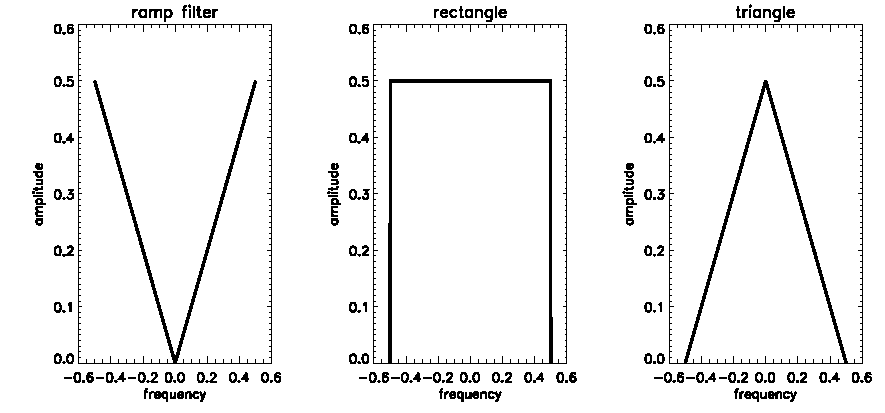
\includegraphics[width=\figmedium]{figs/fig_rampfilter2_app.pdf}
\caption{\label{fig:rampapp2} \emph{The ramp filter can be computed as
    the difference between a rectangular and a triangular filter}}
\end{figure}

Consider the rectangular filter ${\cal R}(\omega)$ of figure  \ref{fig:rampapp2}: its
value equals $W$ for frequency $\omega$ between $-W$ and $W$, and it is
zero elsewhere. Its inverse Fourier transform equals:
\begin{eqnarray}
R(x) & = & W \int_{-\infty}^{\infty} {\cal R}(\omega) e^{2\pi j \omega x} 
           d\omega \nonumber\\
 &=& W \int_{-W}^W e^{2\pi j \omega x} d\omega 
   \hspace{5mm} = \hspace{5mm} 
     W \int_{-W}^W (\cos(2\pi \omega x) + j \sin(2\pi \omega x)) d\omega 
       \nonumber\\
 &=& W \int_{-W}^W \cos(2\pi \omega x) d\omega \nonumber\\
 & = & W \frac{\sin(2\pi W x)}{\pi x} 
\end{eqnarray}
The third equality follows from the fact that the integral of a sine
over an interval symmetrical about zero is always zero. The inverse
Fourier of a rectangular filter is a so-called sinc function.

The convolution of a rectangular function with itself is a triangular
function. More precisely, consider the rectangular function 
${\cal R}_2(\omega)$ and the triangular function ${\cal T}(\omega)$
defined as:
\begin{eqnarray}
 {\cal R}_2(\omega) &=& 1 \hspace{5mm} \mbox{if   $-W/2 < \omega < W/2$}
                        \nonumber \\
                    &=& 0  \hspace{5mm} \mbox{otherwise}\\
 {\cal T}(\omega) &=& W - |\omega| \hspace{5mm} 
             \mbox{if   $-W < \omega < W$} \nonumber\\
                  &=& 0  \hspace{5mm} \mbox{otherwise}
\end{eqnarray}
Then it is easy to verify that the convolution of ${\cal R}_2(\omega)$
with itself equals ${\cal T}(\omega)$:
\begin{eqnarray}
    \int_{-\infty}^\infty {\cal R}_2(\omega') 
                          {\cal R}_2(\omega - \omega') d\omega'
&=& \int_{-W/2}^{W/2} {\cal R}_2(\omega - \omega') d\omega' \nonumber\\
&=& \int_{\omega-W/2}^{\omega+W/2} {\cal R}_2(\omega') d\omega' \nonumber\\
&=& {\cal T}(\omega) 
\end{eqnarray}
Note that the rectangular filters ${\cal R}_2(\omega)$ and ${\cal
R}(\omega)$ have a different width and amplitude.

Convolution in the Fourier transform corresponds to a product in the
spatial domain, so the inverse Fourier transform of a triangular
filter is the square of a sinc function. Therefore, the inverse
Fourier transform of the difference between the rectangular and
triangular filters, i.e. the ramp filter, equals:
\begin{equation}
  W \frac{\sin(2 \pi W x)}{\pi x} - \frac{\sin^2(\pi W x)}{(\pi x)^2}.
  \label{eq:ramp}
\end{equation}

Figure \ref{fig:rampapp} shows a plot of (\ref{eq:ramp}). In a
discrete implementation, where one only needs the function values at
integer positions $x = -N, -N+1, \ldots,N$, the highest possible value
for $W$ is 0.5, the Nyquist frequency. The red dots in the figure show
these discrete function values for $W = 0.5$. 

\begin{figure}[tb]
\centering
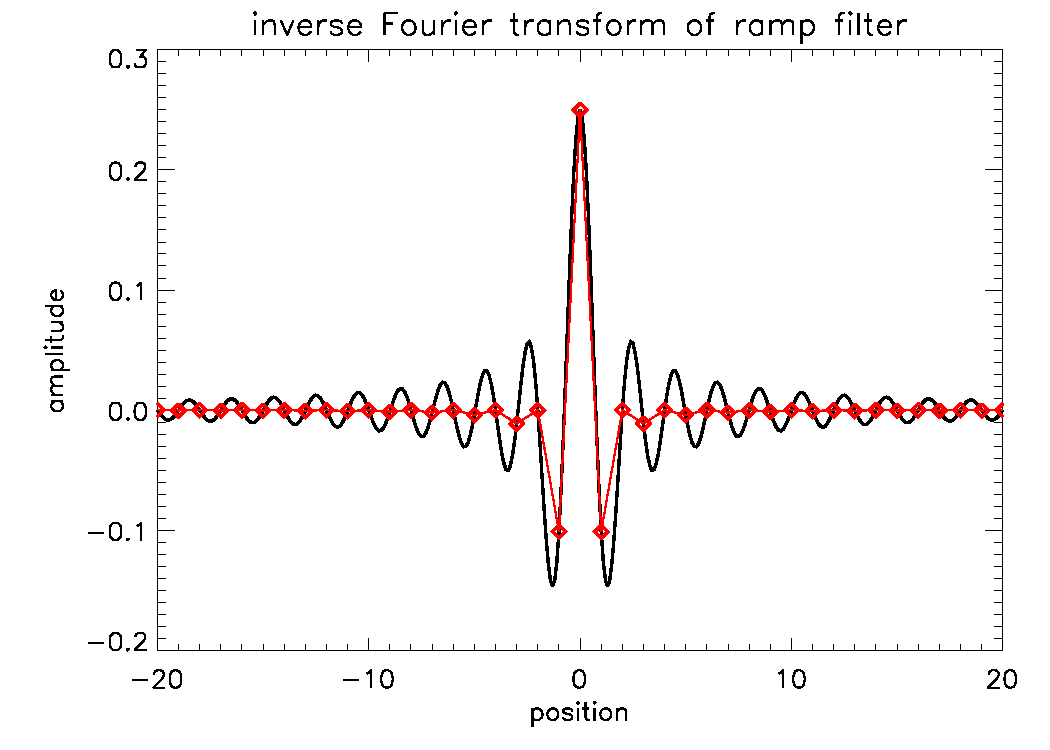
\includegraphics[width=\figmedium]{figs/fig_rampfilter_app.pdf}
\caption{\label{fig:rampapp} \emph{The inverse Fourier transform of
    the ramp filter, with a fine sampling (black curve). Also shown is
    the sampling of the usual discretisation (red dots).}}
\end{figure}


\newpage
\section{The Laplace transform \label{app:laplace}}
%=========================
The Laplace transform is defined as:
\begin{equation}
  {\cal L} F(t) = f(s) = \int_0^\infty e^{-st} F(t) dt.
\end{equation}
%
The Laplace transform is very useful in computations involving differential
equations, because integrals and derivatives with respect to $t$ are
transformed to very simple functions of $s$. Some of its interesting features
are listed below (most are easy to prove). The functions of the time are at
the left, the corresponding Laplace transforms are at the right:
\begin{eqnarray}
F(t)                        & \Longleftrightarrow & f(s) \\
\frac{dF(t)}{dt}            & \Longleftrightarrow & s f(s) - F(0) \\
e^{at} F(t)                 & \Longleftrightarrow & f(s - a)\\
\int_0^t F(u) G(t - u) du   & \Longleftrightarrow & f(s) g(s) \label{eq:lap1}\\
\int_0^t F(u) du            & \Longleftrightarrow & \frac{f(s)}{s}\\
1                           & \Longleftrightarrow & \frac{1}{s}\\
e^{at}                      & \Longleftrightarrow & \frac{1}{s - a} \label{eq:lap2}
\end{eqnarray}

By combining (\ref{eq:lap1}) and (\ref{eq:lap2}) one obtains
\begin{eqnarray}
\int_0^\infty F(u) e^{-a(t - u)} du & \Longleftrightarrow & \frac{f(s)}{s-a}
\end{eqnarray}